\hoofdstuk{Introduction}

\paragraaf{Problem statement}
%Lunatech has had requests from customers for the development of cross-platform mobile applications. Currently these applications are being developed using webtechnologies such as HTML5 and Javascript. 

%To meet their customer's demands Lunatech has developed cross-platform mobile applications using webtechnologies such as HTML and Javascript. A mobile application developed this way is refered to as webapp because it runs in a browser based environment and is often hosted at a webserver rather than downloaded to the device itself.
%\footnote{Note: when mentioning the word 'current', it refers to the old situation as the process to get to the actual current situation is being illustrated}
To meet their customer's demands, Lunatech needs to develop cross-platform mobile applications. Currently these applications are being developed using web technologies such as HTML and Javascript. A mobile application developed this way is referred to as web app because it runs in a browser based environment and is often hosted at a web server rather than downloaded to the device itself.


The chosen solution the user interface components are built in HTML


The problem with web apps is that they lack in user experience. This is mainly due to the browsers' sandbox environment in which the app runs. Every platform has its own set of recognizable user interface elements, but these cannot be accessed from within the browser environment. To overcome this problem web app built their user interface from HTML.  As a result of this the app will feel not native to the user because its' style does not match the rest of the platform. Web app developers often try to mimic the native look-and-feel but a web app does not live up to the level of user experience a native which application offers. 

%This is mainly due to manner in which user interface components are built in HTML. Every platform has its own set of recognizable elements, but these cannot be accessed from within the browser environment. As a result of this the app will feel not native to the user because its' style does not match the rest of the platform. Webapp developers often try to mimic the native look-and-feel but a webapp does not live up to the level of user experience a native which application offers. 

The direct alternative to web apps are native apps, native are written using technologies proprietary to each platform, hence the term 'native'. What these applications lack in terms of cross-platform support they make up in terms of user experience.  A native app has access to all the platforms proprietary libraries and can rely on the user interface elements provided through these libraries.

Lunatech would like to know how to make use of the look-and-feel from native apps with the cross-platform support of web apps.

\paragraaf{Research questions}

Main research question:
\begin{itemize}
\item \emph{How to develop a cross-platform mobile application while retaining the native look-and-feel?}
\end{itemize}

\noindent Sub research questions:
\begin{itemize}
% \item \emph{Which mobile platforms should be targetted for cross-platform mobile application development?}
% \item \emph{How is the native look-and-feel defined?}
\item \emph{Which solutions to cross-platform mobile application development currently exist?}
\item \emph{Which of these solutions offer the defined native look-and-feel?}
\item \emph{Are these solutions viable for commerical useage?}
\item \emph{Is it viable to implement a custom solution to cross-platform mobile application development?}
\end{itemize}

\paragraaf{Research method}

This paragraph will describe the method used during the research.\\

First the context of the main research question needs to be determined by defining the concepts \emph{native look-and-feel} and \emph{cross-platform}. The \emph{native look-and-feel} is defined by the a set of criteria related to the user experience while \emph{cross-platform} is defined as the scope of which platforms should be targeted.

% Once the concepts in main research question are fully defined the possiblity to look for existing solutions opens up.

% First the \emph{native look-and-feel} needs to be defined. After which it's nessecary to define the scope of \emph{cross-platform} by determining which platforms should be targetted.

% Orgin: Once the concepts in main research question are defined it is needed to research which solutions fit within the context.
% A. Once the scope in main research question has been defined it is needed to research which solutions fit within the scope.
% B. Once the context of main research question has defined it is needed to research which solutions fit within the its scope

Once the context of the main research question has been defined it is needed to research which solutions fit within the its scope. During a preliminary research a market survey will have to be performed in order to determine which solutions to cross-platform app development are available on todays market. Each found solution will be given a closer look and categorized based on requirements provided by Lunatech. Once the categorization is complete the solutions will be filtered based on how far the requirements have been met.

A comparison test will be performed in order to determine which solution is potentially viable for commercial use by Lunatech. This test will consist of a short analysis per solution based on Lunatechs' criteria, and a practical part where a benchmark application will be built. The results will be compared and the solution which offers the most complete set of features will be deemed potentially viable for commercial use by Lunatech. At this point a decision has to be made whether to continue with the potentially viable existing solution or research a custom solution. 

To determine if the chosen solution is viable for commercial use by Lunatech a case study will be performed based on a realistic scenario Lunatech might encounter. During this case study the solution will be analyzed and evaluated.

The results of the case study and the analysis will contribute to answering the main research question. In addition to answering the main research question an recommendation will be given to Lunatech regarding the possible adaptation of the solution for commercial usage.

%todo methode verantwoording.

\newpage
\begin{centering}
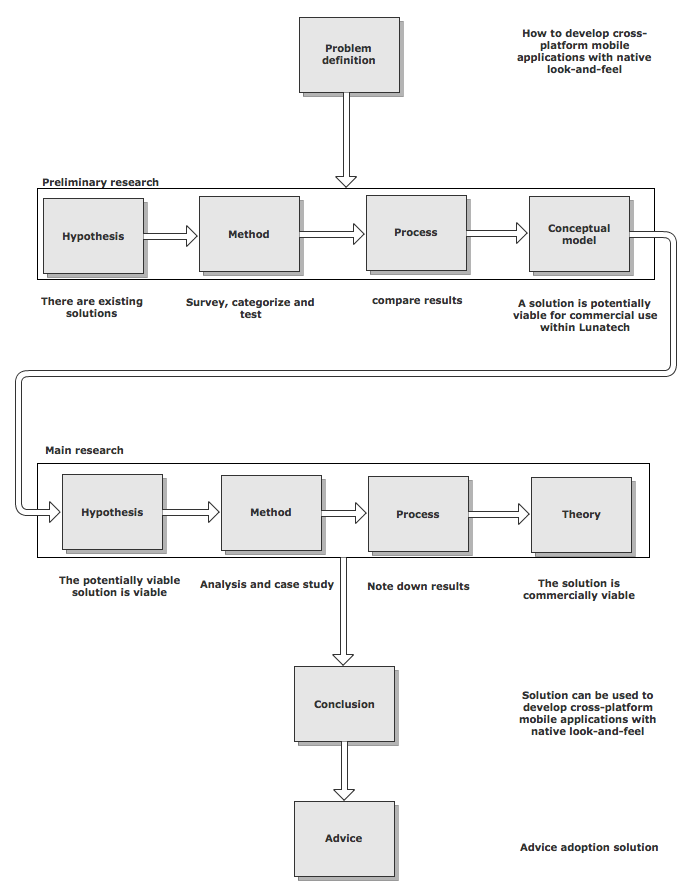
\includegraphics[scale=0.6]{images/researchprocess.png}\\{Research method diagram}\\
\end{centering}

%verantwoorden: why it works analysis. + verantwoorden niet naar andere oplossingen kijken.

